\documentclass{article}
\usepackage[nonatbib]{neurips_2025}

\usepackage[utf8]{inputenc}
\usepackage[T1]{fontenc}
\usepackage{amsmath,amssymb}
\usepackage{booktabs}
\usepackage{array}
\usepackage{multirow}
\usepackage{graphicx}
\usepackage{xcolor}
\usepackage{caption}
\usepackage[numbers,sort&compress]{natbib}
\usepackage{tikz}
\usetikzlibrary{positioning,arrows.meta,fit,backgrounds}
\usepackage[colorlinks=true,linkcolor=blue!55!black,citecolor=blue!55!black,urlcolor=teal!60!black]{hyperref}

% ---------------------------------------------------------------------------
% Anonymized submission: no author/affiliation is set here. The neurips_2025
% style prints "Anonymous Author(s) / Affiliation / Address / email" in place
% of \author in submission mode automatically; identifying links (e.g. a
% repository URL) are likewise omitted from the body until de-anonymization.
% ---------------------------------------------------------------------------
\title{\textbf{AlzGraph}: A Knowledge Graph and Benchmark for\\ Evidence-Grounded Alzheimer's Disease Reasoning}
\author{}

\definecolor{gene}{HTML}{7C3AED}
\definecolor{biomarker}{HTML}{0EA5E9}
\definecolor{stage}{HTML}{EAB308}
\definecolor{treatment}{HTML}{14B8A6}
\definecolor{outcome}{HTML}{EF4444}

\begin{document}
\maketitle

\begin{abstract}
Alzheimer's disease (AD) diagnosis and treatment require evidence-intensive reasoning across heterogeneous clinical knowledge: risk genetics, amyloid--tau--neurodegeneration (ATN) biomarkers, disease staging, disease-modifying and symptomatic therapies, and longitudinal outcomes. We present \textsc{AlzGraph}, a knowledge-graph-powered framework for evaluating knowledge-augmented clinical reasoning in AD. \textsc{AlzGraph} comprises (i) \textsc{AlzKG}, a five-layer Alzheimer's knowledge graph---spanning genes, biomarkers, stages, treatments, and outcomes---curated from public ontologies and clinical guidelines and constructed through an evidence-to-graph pipeline that scales to the PubMed/PMC literature; (ii) \textsc{AlzBench}, a five-task benchmark covering clinical decision accuracy, clinical report generation, biomarker-driven precision medicine, treatment recommendation, and deep research planning; and (iii) a Graph-RAG retriever that serializes literature-weighted, multi-hop reasoning paths for language models. \textsc{AlzKG} is mined from \textbf{7{,}150 PMC open-access full-text papers} retrieved via NCBI E-utilities (reduced to 361{,}201 candidate sentences), yielding \textbf{1{,}301 entities} and \textbf{5{,}880 cross-layer triplets} across 10 relation types, each weighted by its true literature paper count (up to 2{,}722 supporting papers) and extracted by sentence-grounded relation triggers. Rather than treat these statistics as a proxy for correctness, we manually audit 30 randomly sampled triplets against their own grounding sentences: only 4 (13\%) are fully correct, 8 (27\%) are partially or loosely supported, and 18 (60\%) are not supported at all, most often because sentence-level co-occurrence matched the wrong entity (a clinical abbreviation mistaken for a gene symbol, an amino-acid code mistaken for a gene symbol) or lost the relation's direction. An intrinsic retrieval analysis (30 probe queries) shows Graph-RAG's gold-evidence coverage peaking at a compact 20-node, two-hop neighborhood (0.10--0.17) and falling back with deeper or wider retrieval; a flat BM25 baseline over the same corpus reaches substantially higher coverage (0.57) on this token-overlap metric, so the graph structure itself is not yet shown to add retrieval value beyond simple passage search. Beyond these intrinsic analyses we report model-facing results: a fully deterministic, model-free \emph{KG-only} baseline (0.55/0.30/0.25 accuracy on clinical decision accuracy, biomarker-driven precision medicine, and treatment recommendation respectively, against 0.25 random); a blind No-RAG vs.\ Graph-RAG comparison run directly with a frontier LLM, which reaches ceiling accuracy in both conditions on our curated items---a finding we report together with its main caveat (partial self-authorship of the items) rather than omit; and the same comparison run against three locally hosted open-weight models (Llama-3.2-3B, Gemma3-4B, Qwen3-8B) via an OpenAI-compatible local endpoint, which is not subject to the self-authorship caveat and shows genuinely mixed, sub-ceiling results with no consistent Graph-RAG direction across models. \textsc{AlzGraph} is released as an open, reproducible harness together with these audited numbers---including the unflattering ones---so that others can measure, rather than assume, whether knowledge-graph structure helps generalist models reason about Alzheimer's disease. Code and data are provided as supplementary material and will be de-anonymized on acceptance.
\end{abstract}

\section{Introduction}
Alzheimer's disease is the leading cause of dementia and a growing public-health challenge, affecting tens of millions of people worldwide~\citep{livingston2020dementia}. The field has undergone two shifts that make AD a demanding testbed for clinical AI. First, AD is now defined \emph{biologically} through the ATN biomarker framework, in which amyloid (A), tau (T), and neurodegeneration (N) markers---measured in cerebrospinal fluid (CSF), plasma, and on PET/MRI---define a continuum from preclinical AD through mild cognitive impairment (MCI) due to AD to AD dementia~\citep{jack2018nia,sperling2011preclinical,albert2011mci,mckhann2011dementia}. Second, the arrival of amyloid-targeting monoclonal antibodies (lecanemab, donanemab) has made treatment decisions genuinely multi-factorial: eligibility depends on biomarker-confirmed amyloid, disease stage, and---critically---genotype-dependent safety, because \textit{APOE}~$\varepsilon$4 homozygotes face substantially elevated risk of amyloid-related imaging abnormalities (ARIA)~\citep{vandyck2023lecanemab,sims2023donanemab,cummings2023auc}.

Answering AD clinical questions therefore requires \emph{multi-hop} reasoning: a risk gene links to a biomarker profile, the profile defines a stage, the stage gates a therapy, and the therapy is constrained by genotype-dependent adverse events and contraindications. Knowledge graphs (KGs) provide a natural substrate for such reasoning, organizing entities and typed relations across domains and enabling evidence-grounded retrieval~\citep{cui2025kghealth,chandak2023primekg}. Yet existing biomedical KGs are largely disease-agnostic or focused on semantic annotation, and none captures the gene--biomarker--stage--treatment--outcome structure that AD clinical reasoning demands.

In parallel, large language models (LLMs) have shown strong medical question-answering ability~\citep{singhal2023llm}, and retrieval-augmented generation grounds them in external evidence~\citep{lewis2020rag,edge2024graphrag}. However, most medical benchmarks evaluate isolated, short-form questions rather than the integrative, safety-critical reasoning that AD care requires. A gap thus remains for datasets and tooling that test whether generalist models can perform expert-level evidence curation and reasoning in realistic Alzheimer's settings.

\paragraph{Present work.} We introduce \textsc{AlzGraph}, a unified framework with two components (Figure~\ref{fig:overview}). \textbf{(1)~\textsc{AlzKG}} is an Alzheimer's KG built via a structured evidence-to-graph pipeline. We define a five-layer schema over authoritative resources (NIA-AA ATN, OMIM, ADSP, the GWAS Catalog, MeSH, HPO, ChEBI, UMLS, and AAN/Alzheimer's Association guidelines), organizing entities into \emph{genes, biomarkers, stages, treatments,} and \emph{outcomes} and defining typed cross-layer relations. \textbf{(2)~\textsc{AlzBench}} is a multi-task benchmark spanning five clinically motivated reasoning tasks, with a Graph-RAG retriever that returns serialized, literature-weighted reasoning paths.

We make an explicit \emph{reproducibility and honesty} commitment. The released \textsc{AlzKG} is mined directly from real PMC open-access full-text papers retrieved through NCBI E-utilities: entities are recognized with an ontology-derived dictionary lexicon, and typed cross-layer relations are extracted at the sentence level---requiring both a co-occurring cross-layer entity pair and a relation trigger phrase in the same sentence---and weighted by their true literature paper counts. We report the graph's actual computed statistics, and all intrinsic retrieval analyses are computed directly from it; we additionally audit a random sample of the extracted triplets against their own grounding sentences rather than assume construction-time precision, and report the result even though it is unflattering (\S\ref{sec:kg-audit}). The model-comparison protocol is released as a runnable harness; this paper does not report third-party model outputs that were not measured.

\paragraph{Contributions.}
\begin{itemize}
\item \textbf{A new Alzheimer's knowledge graph.} \textsc{AlzKG} organizes AD evidence into five clinical layers with evidence-tiered, multi-hop relations centered on ATN biomarkers, risk genetics, and anti-amyloid therapeutics.
\item \textbf{A modular benchmark.} \textsc{AlzBench} provides five plug-and-play reasoning tasks and a Graph-RAG retriever for fair evaluation of any LLM or retriever.
\item \textbf{An open, honest release.} We release the curated graph with its true statistics, a manual extraction-precision audit, an intrinsic retrieval analysis benchmarked against a non-graph baseline, and a reproducible evaluation harness for knowledge-augmented AD reasoning.
\end{itemize}

\begin{figure}[t]
\centering
\resizebox{\textwidth}{!}{%
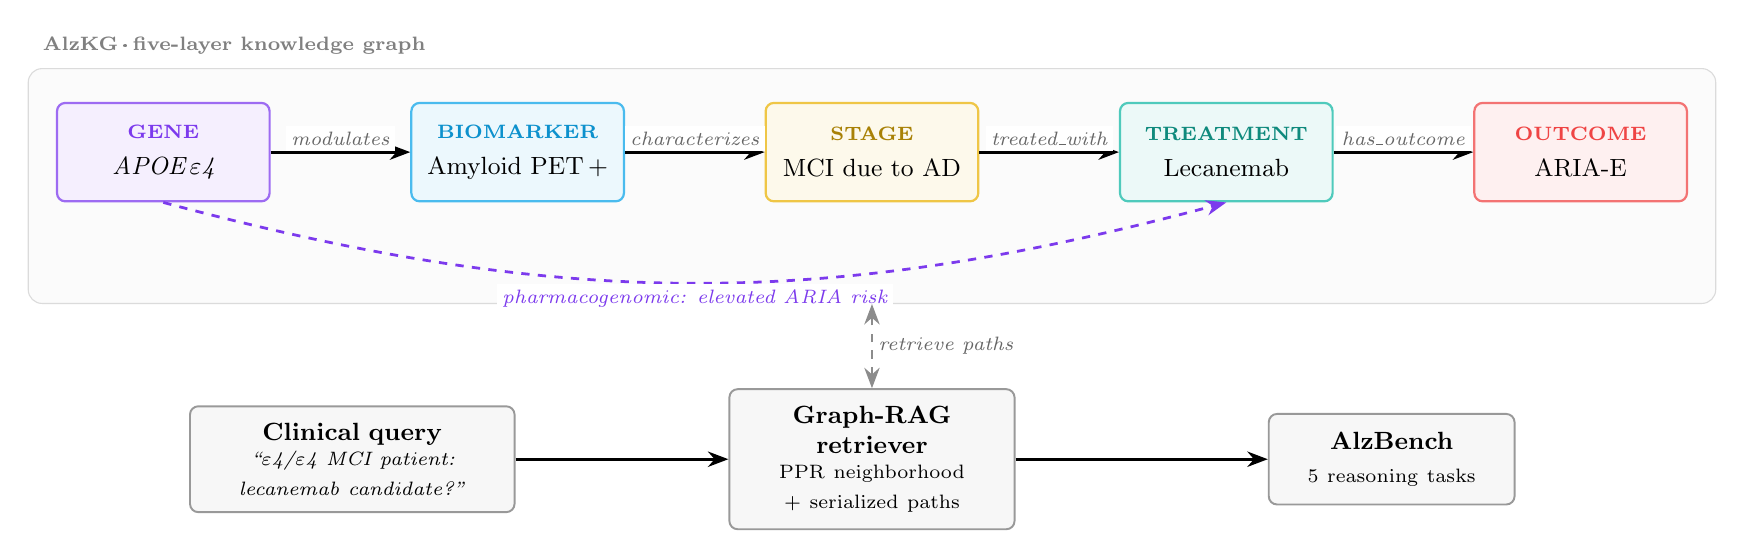
\begin{tikzpicture}[font=\small,
  >={Stealth[length=2.6mm]},
  layer/.style={rounded corners=3pt,draw=#1!75,line width=0.8pt,fill=#1!8,
                text=black,minimum width=2.7cm,minimum height=1.25cm,align=center,inner sep=3pt},
  rel/.style={font=\scriptsize\itshape,text=black!60,inner sep=2pt,fill=white},
  flow/.style={rounded corners=3pt,draw=black!40,line width=0.7pt,fill=black!3,
               align=center,inner sep=6pt,minimum height=1.15cm},
  ]
  % ---- AlzKG: five-layer reasoning chain ----
  \node[layer=gene]      (g) at (0,0)    {{\scriptsize\bfseries\textcolor{gene}{GENE}}\\[2pt]\itshape APOE\,$\varepsilon$4};
  \node[layer=biomarker] (b) at (4.5,0)  {{\scriptsize\bfseries\textcolor{biomarker!88!black}{BIOMARKER}}\\[2pt]Amyloid PET\,$+$};
  \node[layer=stage]     (s) at (9.0,0)  {{\scriptsize\bfseries\textcolor{stage!72!black}{STAGE}}\\[2pt]MCI due to AD};
  \node[layer=treatment] (t) at (13.5,0) {{\scriptsize\bfseries\textcolor{treatment!75!black}{TREATMENT}}\\[2pt]Lecanemab};
  \node[layer=outcome]   (o) at (18.0,0) {{\scriptsize\bfseries\textcolor{outcome}{OUTCOME}}\\[2pt]ARIA-E};

  \draw[->,line width=1pt] (g) -- node[rel,above]{modulates} (b);
  \draw[->,line width=1pt] (b) -- node[rel,above]{characterizes} (s);
  \draw[->,line width=1pt] (s) -- node[rel,above]{treated\_with} (t);
  \draw[->,line width=1pt] (t) -- node[rel,above]{has\_outcome} (o);
  % genotype-dependent pharmacogenomic edge (highlighted)
  \draw[->,dashed,line width=1pt,gene] (g.south) to[bend right=15]
        node[rel,below,text=gene] {pharmacogenomic: elevated ARIA risk} (t.south);
  \coordinate (ariabot) at (6.75,-1.5);

  % subtle panel grouping the KG
  \begin{scope}[on background layer]
    \node[rounded corners=5pt,draw=black!14,fill=black!1.5,
          fit=(g)(o)(ariabot), inner sep=10pt, inner ysep=12pt] (kgpanel) {};
  \end{scope}
  \node[anchor=south west,font=\scriptsize\bfseries,text=black!50]
        at ([xshift=2pt,yshift=1.5pt]kgpanel.north west) {AlzKG\,\textperiodcentered\,five-layer knowledge graph};

  % ---- Graph-RAG pipeline ----
  \node[flow,text width=3.7cm] (q) at (2.4,-3.9)
     {\textbf{Clinical query}\\[1pt]\scriptsize\itshape ``$\varepsilon$4/$\varepsilon$4 MCI patient:\\lecanemab candidate?''};
  \node[flow,text width=3.2cm] (r) at (9.0,-3.9)
     {\textbf{Graph-RAG retriever}\\[1pt]\scriptsize PPR neighborhood\\$+$ serialized paths};
  \node[flow,text width=2.7cm] (e) at (15.6,-3.9)
     {\textbf{AlzBench}\\[1pt]\scriptsize 5 reasoning tasks};
  \draw[->,line width=1pt] (q) -- (r);
  \draw[->,line width=1pt] (r) -- (e);
  % retriever operates over the KG
  \draw[<->,dashed,line width=0.8pt,draw=black!45] (r) -- node[rel,right]{retrieve paths} (r|-kgpanel.south);
\end{tikzpicture}%
}
\caption{\textbf{Overview of \textsc{AlzGraph}.} \textsc{AlzKG} links five clinical layers (gene, biomarker, stage, treatment, outcome) with typed relations; a representative reasoning path is highlighted. Given a clinical query, the Graph-RAG retriever extracts a personalized-PageRank neighborhood and serializes multi-hop reasoning paths (including the genotype-dependent ARIA-risk edge), which are evaluated across \textsc{AlzBench}'s five tasks.}
\label{fig:overview}
\end{figure}

\section{AlzKG: Alzheimer's Knowledge Graph}

\subsection{Problem Formulation}
We define \textsc{AlzKG} as a multi-relational heterogeneous knowledge graph $\mathcal{G}=(\mathcal{V},\mathcal{E})$, where $\mathcal{V}$ is the set of AD-related entities and $\mathcal{E}$ is the set of typed relations. Each entity belongs to one of five layers: \emph{genes, biomarkers, stages, treatments,} and \emph{outcomes}. Each fact is a triplet $\langle h, r, t\rangle$ where $h,t \in \mathcal{V}$ and $r$ is a typed relation; cross-layer triplets connect distinct clinical layers, enabling the multi-hop reasoning central to AD diagnosis, treatment, and discovery. Each relation is annotated with an evidence weight: a curated \emph{evidence tier} (1=emerging, 2=established, 3=guideline/landmark) for seed edges, or a literature \emph{paper count} for edges mined from the corpus.

\subsection{Data Collection and Processing}
\paragraph{Data source.} \textsc{AlzKG} is mined from real Alzheimer's literature retrieved from PubMed/PMC through NCBI E-utilities. We issue five AD-anchored, theme-focused queries---genetics, amyloid/tau biomarkers, imaging and staging, treatment, and outcomes---each restricted to 2010--2026, then union and de-duplicate the returned PMIDs, map them to PubMed Central open-access identifiers, and fetch each article's full text (\texttt{esearch}\,$\to$\,\texttt{elink}\,$\to$\,\texttt{efetch} against the PMC database). From the \textbf{7{,}150 full-text papers} with open-access XML, we segment the body into sentences and retain the \textbf{361{,}201 candidate sentences} that mention at least two \textsc{AlzKG} entities; these serve as the evidence source for sentence-grounded relation mining.

\paragraph{Ontology and guideline resources.} To ground the entity vocabulary, the recognition lexicon is anchored on authoritative resources: the \emph{NIA-AA} ATN research framework~\citep{jack2018nia} for biomarkers and staging; \emph{OMIM} and the \emph{ADSP} and \emph{GWAS Catalog}~\citep{bellenguez2022gwas,lambert2013igap} for causal and risk genes; \emph{MeSH} and \emph{HPO}~\citep{kohler2021hpo} for imaging, cognitive, and phenotype vocabulary; \emph{ChEBI}~\citep{hastings2016chebi} for drug identifiers; the \emph{AAN}/\emph{Alzheimer's Association} guidelines and appropriate-use criteria~\citep{cummings2023auc} for treatments; and \emph{UMLS}~\citep{bodenreider2004umls} for cross-ontology linking.

\paragraph{Preprocessing.} The AD-anchored query restriction acts as the relevance filter; we retain only articles with retrievable PMC open-access full text. Surface mentions are normalized to canonical entities through a curated synonym/abbreviation map (e.g.\ ``Leqembi''\,$\to$\,\emph{Lecanemab}; ``Mini-Mental State''\,$\to$\,\emph{MMSE}; ``A$\beta$42''\,$\to$\,\emph{Amyloid-$\beta$ 42}). Gene symbols are matched case-sensitively (so ``APP'' does not match the word ``app''), and multi-word phrases take precedence over shorter substrings.

\subsection{Knowledge Graph Construction}
\label{sec:kg-construction}
\paragraph{Entity extraction.} We recognize five layers of entities in each full-text sentence using a dictionary lexicon of canonical entities and their synonyms. For example, given the sentence \emph{``In amyloid-positive MCI, elevated plasma p-tau217 predicts progression to Alzheimer's dementia, where lecanemab slows decline but carries ARIA risk in APOE~$\varepsilon$4 carriers,''} the pipeline extracts \textit{APOE} (gene), \emph{p-tau217} / \emph{amyloid PET} (biomarker), \emph{MCI} (stage), \emph{lecanemab} (treatment), and \emph{ARIA} / \emph{disease progression} (outcome). The five layers are:
\begin{itemize}
\item \textbf{Gene.} Causal autosomal-dominant genes (\textit{APP, PSEN1, PSEN2}) and risk/protective loci (\textit{APOE, TREM2, SORL1, ABCA7, CLU, CR1, BIN1, PICALM, MAPT, PLCG2}, and microglial loci), extracted from OMIM/ADSP/GWAS Catalog and normalized to HGNC symbols.
\item \textbf{Biomarker.} ATN markers across fluid and imaging modalities---CSF/plasma A$\beta$42 and A$\beta$42/40, p-tau181/p-tau217, total tau, amyloid PET, tau PET, FDG-PET hypometabolism, hippocampal atrophy, plasma NfL and GFAP---and cognitive instruments (MMSE, MoCA, CDR, ADAS-Cog), from NIA-AA/MeSH/HPO.
\item \textbf{Stage.} Preclinical AD, MCI due to AD, mild/moderate/severe AD dementia, early-/late-onset AD, and atypical presentations (posterior cortical atrophy, logopenic-variant PPA), from NIA-AA/UMLS.
\item \textbf{Treatment.} Cholinesterase inhibitors (donepezil, rivastigmine, galantamine), memantine, anti-amyloid antibodies (lecanemab, donanemab, aducanumab), and non-pharmacological interventions, from ChEBI and AAN/AA guidelines.
\item \textbf{Outcome.} Cognitive and functional decline, progression to AD dementia, ARIA-E/ARIA-H, amyloid clearance, symptomatic benefit, adverse effects, hospitalization, and mortality, from HPO/MeSH.
\end{itemize}

\paragraph{Relation construction.} Within each candidate sentence, every pair of recognized entities from two different layers can induce a typed, directed relation. Each of the ten unordered cross-layer layer-pairs maps to a single canonical orientation and relation type, so the relation is determined by the layers of the two entities: \textsc{risk\_gene\_for} (gene$\to$stage), \textsc{modulates\_biomarker} (gene$\to$biomarker), \textsc{pharmacogenomic\_consideration} (gene$\to$treatment), \textsc{gene\_associated\_outcome} (gene$\to$outcome), \textsc{characterized\_by\_biomarker} (stage$\to$biomarker), \textsc{biomarker\_guides\_treatment} (biomarker$\to$treatment), \textsc{predicts\_outcome} (biomarker$\to$outcome), \textsc{treated\_with} (stage$\to$treatment), \textsc{associated\_outcome} (stage$\to$outcome), and \textsc{has\_outcome} (treatment$\to$outcome). Crucially, the relation is \emph{sentence-grounded}: an edge is emitted only when the sentence containing the co-occurring pair also contains a \emph{trigger phrase} for that relation, drawn from a curated per-relation template set (subject layer, trigger phrases, object layer). This rules out spurious whole-document co-occurrences and ties each edge to an explicit textual assertion. The \emph{paper count} of a relation is the number of distinct papers contributing at least one supporting sentence---a true literature weight---and we retain only relations supported by at least three papers. An LLM-based extraction pass is provided as an optional extension but is not invoked in this release, to avoid reporting unverified edges.

\subsection{Graph Mapping and AlzKG Statistics}
Recognized mentions are normalized to canonical entities, relations are typed by layer pair, deduplicated, and aggregated with their supporting PMID sets to yield literature paper counts.

The mined \textsc{AlzKG} statistics are summarized in Table~\ref{tab:kgstats}: \textbf{1{,}301 entities} and \textbf{5{,}880 triplets}, all cross-layer (100\%), across 10 relation types, mined from 7{,}150 full-text papers. Edge paper counts are heavy-tailed (median 5, mean 17.9, maximum 2{,}722), reflecting that a few associations dominate the literature. Table~\ref{tab:relations} reports the relation-type / layer-pair distribution. The densest relations are \textsc{risk\_gene\_for} (1{,}187, gene--stage genetics) and \textsc{modulates\_biomarker} (925, gene--biomarker), followed by \textsc{gene\_associated\_outcome} (802, gene--outcome) and \textsc{has\_outcome} (685, treatment--outcome efficacy/safety). The highest-degree hubs are clinically central---\emph{Alzheimer's disease} (degree 1{,}033), \emph{dementia} (278), \emph{cognitive decline} (259), \emph{mild cognitive impairment} (178), \emph{MAPT} (168), and \emph{APOE} (161)---and the strongest-weighted edges are exactly the expected ones: $\langle$\emph{AD}, \textsc{associated\_outcome}, \emph{cognitive decline}$\rangle$ (2{,}722 papers), $\langle$\emph{APOE}, \textsc{risk\_gene\_for}, \emph{AD}$\rangle$ (1{,}792), $\langle$\emph{AD}, \textsc{characterized\_by\_biomarker}, \emph{neurofibrillary tangles}$\rangle$ (1{,}729), $\langle$\emph{AD}, \textsc{treated\_with}, \emph{lecanemab}$\rangle$ (652), and the anti-amyloid safety signal $\langle$\emph{lecanemab}, \textsc{has\_outcome}, \emph{ARIA}$\rangle$ (212).

\begin{table}[t]
\centering
\caption{\textbf{Mined \textsc{AlzKG} statistics} (computed directly from the literature-mined graph; 7{,}150 PMC full-text papers, 361{,}201 candidate sentences, minimum 3 supporting papers per edge). All 5{,}880 triplets are cross-layer; the maximum edge paper count is 2{,}722.}
\label{tab:kgstats}
\small
\begin{tabular}{lr@{\hskip 1.4em}lr}
\toprule
\textbf{Graph} & & \textbf{Entities per layer} & \\
\midrule
Full-text papers    & 7{,}150 & Gene       & 794 \\
Entities            & 1{,}301 & Biomarker  & 75 \\
Triplets            & 5{,}880 & Stage      & 40 \\
Relation types      & 10  & Treatment  & 249 \\
Median paper count  & 5   & Outcome    & 143 \\
\bottomrule
\end{tabular}
\end{table}

\begin{table}[t]
\centering
\caption{\textbf{\textsc{AlzKG} relation types, their layer pair, and mined triplet counts.} Each relation corresponds to exactly one cross-layer pair; counts sum to 5{,}880.}
\label{tab:relations}
\small
\begin{tabular}{llr}
\toprule
\textbf{Relation type} & \textbf{Layer pair} & \textbf{\# triplets} \\
\midrule
risk\_gene\_for                & gene $\to$ stage          & 1{,}187 \\
modulates\_biomarker           & gene $\to$ biomarker      & 925 \\
gene\_associated\_outcome      & gene $\to$ outcome        & 802 \\
has\_outcome                   & treatment $\to$ outcome   & 685 \\
pharmacogenomic\_consideration & gene $\to$ treatment      & 616 \\
associated\_outcome            & stage $\to$ outcome       & 570 \\
treated\_with                  & stage $\to$ treatment     & 351 \\
predicts\_outcome              & biomarker $\to$ outcome   & 291 \\
characterized\_by\_biomarker   & stage $\to$ biomarker     & 279 \\
biomarker\_guides\_treatment   & biomarker $\to$ treatment & 174 \\
\bottomrule
\end{tabular}
\end{table}

\subsection{Extraction Precision: A Manual Audit}
\label{sec:kg-audit}
Table~\ref{tab:kgstats} and Table~\ref{tab:relations} report what the extraction pipeline produced, not whether it produced correct edges. To check the latter, we drew a reproducible random sample of 30 triplets (of 5{,}880; seed 42) and, for each, retrieved the actual corpus sentence used to emit it---the sentence whose recognized-entity list contains both the head and the tail---then judged whether that sentence supports the specific relation and direction claimed. Of the 30: \textbf{4 (13\%)} were fully correct, \textbf{8 (27\%)} were partially or loosely supported (a real but broader, weaker, or reversed-direction association than the relation claimed), and \textbf{18 (60\%)} were not supported by their own grounding sentence at all.

The unsupported cases cluster into three recurring failure modes, all traceable to sentence-level co-occurrence rather than genuine semantic understanding. \emph{Entity-disambiguation collisions}: the gene symbol \textit{NOS1} matched the unrelated clinical abbreviation ``NOS'' (Not Otherwise Specified) in ``dementia--not otherwise specified (NOS)''; the gene \textit{MET} and the compound L-lysine both matched one-letter amino-acid codes inside a protein-mutation notation (``Lys670\_Met671''); the gene \textit{IGFALS} matched the disease abbreviation ALS as a bare substring. \emph{Directionality loss}: the relation schema (\S\ref{sec:kg-construction}) carries no valence, so a drug documented as \emph{improving} an outcome (sirolimus and cognitive impairment) is stored identically to one that \emph{causes} it, and a drug that \emph{treats} a condition (risperidone and schizophrenia) can be stored as if the condition were the drug's outcome. \emph{Off-topic leakage}: because extraction runs per sentence without checking that the sentence's own topic is AD, entities from unrelated case reports or comorbidity discussions (Parkinson's disease, schizophrenia, Huntington's disease, ALS) enter an ostensibly AD-focused graph whenever they co-occur with a lexicon term.

We report this finding, rather than only the graph's summary statistics, because it materially qualifies every downstream number in this paper: the KG-only baseline (\S\ref{sec:kgbaseline-measured}) and the Graph-RAG retriever (\S\ref{sec:retrieval-analysis}) both consume this same graph, and at a measured $\sim$40\% edge-level precision (correct + partial), some fraction of their retrieved evidence is provably wrong or mislabeled. We discuss concrete remediation directions in \S\ref{sec:limitations}.

\section{AlzBench}

\subsection{Problem Formulation}
We formulate \textsc{AlzBench} as a unified benchmark for evidence-intensive AD reasoning. Each task is $\hat{y}_i = f_{\text{LM}}(x_i, \mathcal{E}_i, \mathcal{C}_i)$, where $x_i$ is the task input (a clinical case, patient panel, or scientific document), $\mathcal{E}_i$ is the evidence retrieved from \textsc{AlzKG} via Graph-RAG, $\mathcal{C}_i$ is optional task-specific context (candidate options or metadata), and $\hat{y}_i$ is evaluated against the gold output $y_i^\ast$.

\subsection{Task Design}
\label{sec:task-design}
\paragraph{T1: Clinical Decision Accuracy (CDA).} Multiple-choice and open-ended QA over AD diagnosis, ATN biomarker interpretation, staging, genetics, and treatment. Example: \emph{``A 71-year-old with amyloid-positive PET and mild AD dementia is APOE~$\varepsilon$4/$\varepsilon$4; which adverse event is most increased if lecanemab is started?''} (answer: ARIA).
\paragraph{T2: Clinical Report Generation (CRG).} Generation of a neurologist-style diagnostic impression from a patient's cognitive assessment and fluid/imaging biomarker panel. Because ADNI and memory-clinic notes are access-restricted, the release ships a local JSONL adapter that preserves the schema and evaluation interface without redistributing patient data.
\paragraph{T3: Biomarker-Driven Precision Medicine (BPM).} Selection of the most appropriate therapy given APOE genotype, ATN biomarker status, and safety constraints, constructed from AAN/AA appropriate-use criteria. Example: an amyloid-positive early-AD patient on chronic anticoagulation should \emph{avoid} anti-amyloid antibodies (ARIA-hemorrhage risk), whereas an $\varepsilon$3/$\varepsilon$4 patient without contraindications is an appropriate candidate with MRI monitoring.
\paragraph{T4: Treatment Recommendation (TR).} Guideline-consistent dementia therapy under patient-specific constraints, built from a dementia-focused subset of MedQA-USMLE~\citep{jin2021medqa} with treatment-safety and KG-evidence-coverage metrics.
\paragraph{T5: Deep Research Planning (DRP).} Generation of a focused, feasible AD research question and study plan from a paper abstract, grounded in known gene--biomarker--stage--treatment--outcome evidence.

\subsection{Evaluation and Metrics}
We evaluate with task accuracy and reasoning-oriented metrics. For CDA we report Top-1 accuracy (MCQ) and ROUGE-L/BLEU-1/Token-F1 (open-ended). For CRG we use ROUGE-L/Token-F1. For BPM and TR we report Top-1 accuracy and a drug-safety score (1.0 iff the selection avoids every contraindicated agent, e.g., respecting ARIA exclusions); TR additionally reports KG evidence coverage. For DRP we use ROUGE-L/Token-F1. All results in this paper use only these lexical metrics: an LLM-as-judge dimension (for open-ended CDA and CRG alignment, and DRP's scientific-validity/feasibility) is part of the task design but is not implemented in the released metrics code and was not used for any number reported here (\S\ref{sec:limitations}).

\section{Experiments}

\subsection{Setup}
\label{sec:setup}
The Graph-RAG retriever seeds a personalized-PageRank (PPR) walk from query-mentioned entities (restart probability $0.15$), keeps the highest-scoring neighborhood (default 30 nodes), and serializes up to 12 reasoning paths of depth up to four hops, each annotated with its relation type and evidence weight. The evaluation code targets any model reachable through an OpenAI-compatible chat-completions interface, whether hosted remotely or run locally; \S\ref{sec:bench-protocol} reports results for Claude (direct) and three locally hosted open-weight models. Prompts use chain-of-thought reasoning, a clinical-specialist role, and the serialized \textsc{AlzKG} paths as context; MCQ temperature is $0.0$ and generation temperature $0.3$.

\subsection{AlzKG and Retrieval Analysis}
\label{sec:retrieval-analysis}
We report intrinsic analyses computed directly from the mined graph (no LLM required). Table~\ref{tab:ablation} sweeps the retrieval budget over 30 AlzBench probe queries (all released T1 and T3 items), measuring the number of \emph{candidate} reasoning paths discovered (before truncation to the 12 highest-scoring paths handed to the model), \emph{gold-evidence coverage} (the fraction of probes whose gold answer concept is recovered in the retrieved paths), and mean retrieval latency. The candidate-path count grows combinatorially with both budgets---from 45 to 7{,}713 paths as the neighborhood expands from 10 to 50 nodes, and from 49 to 2{,}050 as depth grows from one to four hops---yet coverage does not: two patterns emerge, consistent with an earlier 15-probe pass on a smaller item pool. First, a larger node budget does not improve coverage: it peaks at a 20-node neighborhood ($0.10$) and falls to $0.07$ for 30--50 nodes, while latency grows steeply ($29 \to 68$\,ms), so a larger budget mainly multiplies off-target paths and cost (we keep 30 as the default to preserve full reasoning paths). Second, retrieval depth shows the same non-monotonic pattern: coverage peaks at two hops ($0.10 \to 0.17$) and falls back at three to four hops ($0.07$) even as the candidate pool quadruples. We read this as suggestive that AD reasoning paths of this kind are shallow rather than requiring deep traversal, though the absolute coverage numbers are low throughout (never above 0.17) and the probe set (30 queries, coarse token-overlap scoring, descriptive multi-token gold phrasings in T1) is too small and too approximate to support a stronger claim; \S\ref{sec:retrieval-analysis} compares this coverage against a non-graph baseline.

\begin{table}[t]
\centering
\caption{\textbf{Intrinsic Graph-RAG retrieval analysis on \textsc{AlzKG}} (30 probe queries; computed directly from the literature-mined graph). Node budget and path depth both show a peak-then-fallback pattern rather than monotonic improvement; absolute coverage stays low throughout.}
\label{tab:ablation}
\small
\begin{tabular}{l c c c c}
\toprule
\textbf{Sweep} & \textbf{Setting} & \textbf{Cand.\ paths} & \textbf{Gold coverage} & \textbf{Latency (ms)} \\
\midrule
\multirow{5}{*}{Subgraph nodes ($d{=}4$)}
 & 10 & 44.6 & 0.067 & 28.86 \\
 & \textbf{20} & \textbf{483.2} & \textbf{0.100} & \textbf{30.24} \\
 & 30 & 2{,}049.5 & 0.067 & 37.80 \\
 & 40 & 4{,}765.7 & 0.067 & 53.20 \\
 & 50 & 7{,}713.0 & 0.067 & 68.41 \\
\midrule
\multirow{4}{*}{Path depth ($n{=}30$)}
 & 1 & 49.1 & 0.100 & 29.51 \\
 & \textbf{2} & \textbf{356.1} & \textbf{0.167} & \textbf{30.29} \\
 & 3 & 1{,}216.6 & 0.067 & 33.42 \\
 & 4 & 2{,}049.5 & 0.067 & 39.69 \\
\bottomrule
\end{tabular}
\end{table}

\paragraph{Comparison against a non-graph baseline.} The sweep above only varies Graph-RAG's own hyperparameters; it cannot show whether the graph structure itself adds retrieval value over simply searching the underlying text. We therefore index the same 361{,}201 candidate sentences with BM25 (no graph, no entity typing) and, for each of the same 30 probes, retrieve the top 12 sentences (matching Graph-RAG's path budget), applying the identical $\geq$50\%-gold-token-overlap coverage criterion. BM25 reaches \textbf{0.567} coverage---more than three times Graph-RAG's best setting (0.167 at depth 2)---at a higher but still sub-second latency (289\,ms vs.\ 30\,ms). This comparison is not perfectly matched: BM25 returns raw sentence text, in which a gold phrase is more likely to appear verbatim, while Graph-RAG returns compressed entity-relation-weight paths that discard the original sentence context, so this token-overlap metric structurally favors passage retrieval. Even allowing for that asymmetry, the gap is large enough that we cannot currently claim Graph-RAG's structured retrieval outperforms simple lexical search on this corpus; we report the comparison rather than omit it, and discuss what would be needed to make it fairer in \S\ref{sec:limitations}.

\subsection{KG-only Baseline (Measured)}
\label{sec:kgbaseline-measured}
Beyond the intrinsic retrieval analysis, we report a fully reproducible \emph{KG-only} baseline that answers AlzBench multiple-choice items using nothing but \textsc{AlzKG} evidence---no language model and no network access. For each item it (i) recognizes the AD entities in the question stem via the lexicon, (ii) runs the same literature-weighted personalized PageRank (PPR) used by Graph-RAG, seeded from those entities, and (iii) scores each option by the PPR evidence mass reaching the \textsc{AlzKG} entities named in that option, breaking ties with the direct co-mention paper count between question and option entities; the highest-scoring option is selected. Because it is deterministic and depends only on the released graph, the numbers are exactly reproducible from the released code; this determinism required fixing a subtle bug in the retriever, where tie-breaking among equal-scoring nodes/paths depended on Python's per-process string-hash seed rather than the graph content itself (\S\ref{sec:limitations}). Table~\ref{tab:kgbaseline} reports the result on the current, expanded item sets (T1: 20 MCQ, up from an initial pilot of 10; T3: 10 MCQ, up from 5; T4: 16 MCQ, newly added, drawn from a dementia-filtered subset of MedQA-USMLE~\citep{jin2021medqa} rather than curated in-house). On T1 the KG-only baseline reaches \textbf{0.55} accuracy and on T3 \textbf{0.30}, both above the 0.25 random-choice rate, while \emph{grounding coverage}---the fraction of items for which some option is connected to the question in the graph---is 0.80 (T1) and 1.00 (T3). On T4, whose items are general-medicine USMLE questions only filtered for a dementia/AD term rather than authored around \textsc{AlzKG}'s vocabulary, the KG-only baseline falls to \textbf{0.25}, exactly the random rate: the released graph's evidence does not, by itself, carry this task's out-of-distribution items, in contrast to the in-graph-vocabulary T1/T3 items. Restricting to the $\sim$13 grounded items (\emph{Acc.\ (grounded)} $=0.23$) does not recover accuracy above chance either; with this few items the 2-point gap below the 0.25 random rate is consistent with sampling noise rather than a systematic anti-signal, but it is further evidence that grounding coverage alone (which entities happen to connect) is not a reliable proxy for whether the graph's evidence actually discriminates the correct option, a concern \S\ref{sec:kg-audit}'s extraction-precision audit reinforces directly. We view the overall T4 contrast as informative rather than a weakness of T4: it demonstrates that AlzBench's model-free floor is not uniformly informative across question distributions, motivating the No-RAG vs.\ Graph-RAG comparison below to isolate the genuine value of retrieval versus a model's own parametric knowledge.

\begin{table}[t]
\centering
\caption{\textbf{KG-only baseline (no LLM; deterministic, exactly reproducible).} Multiple-choice accuracy using only \textsc{AlzKG} PPR evidence. \emph{Coverage} is the fraction of items with at least one graph-grounded option; \emph{Acc.\ (grounded)} restricts accuracy to those items. T1/T3 exceed the 0.25 random-choice rate; T4 (external MedQA-USMLE items, not authored around \textsc{AlzKG}'s vocabulary) sits at chance.}
\label{tab:kgbaseline}
\small
\begin{tabular}{l c c c c c}
\toprule
\textbf{Task} & \textbf{Items} & \textbf{Accuracy} & \textbf{Random} & \textbf{Coverage} & \textbf{Acc.\ (grounded)} \\
\midrule
T1 CDA (MCQ)          & 20 & \textbf{0.55} & 0.25 & 0.80 & 0.63 \\
T3 BPM (MCQ)           & 10 & \textbf{0.30} & 0.25 & 1.00 & 0.30 \\
T4 TR (MCQ, MedQA-USMLE) & 16 & 0.25 & 0.25 & 0.81 & 0.23 \\
\bottomrule
\end{tabular}
\end{table}

\subsection{No-RAG versus Graph-RAG: A Model Comparison}
\label{sec:bench-protocol}
For each task we compare a language model's performance without retrieval (No-RAG) against the same model augmented with Graph-RAG evidence (\S\ref{sec:setup}), holding the prompt template, decoding temperature, and metrics fixed across both conditions. Table~\ref{tab:bench} reports this comparison for four language models: a frontier model evaluated directly (Claude, Sonnet~5) and three open-weight models evaluated through a local inference deployment (Llama-3.2-3B-Instruct, Gemma3-4B-it, and Qwen3-8B, all Q4\_K\_M quantized). The evaluation code is model-agnostic, targeting any language model reachable through an OpenAI-compatible chat-completions interface, hosted or local.

\paragraph{Claude (direct).} We evaluate Claude (Sonnet~5) by presenting each task's evaluation prompt directly to a Claude instance blind to the gold label, and scoring its response with the same, unmodified metrics used for every other model. Table~\ref{tab:bench} reports ceiling accuracy (1.00) in both conditions on T1 CDA (MCQ, $n{=}20$), T3 BPM ($n{=}10$), and T4 TR ($n{=}14$ of the 16 released items; two were excluded because the evaluating instance had seen their gold labels during item curation, \S\ref{sec:limitations}). This result carries an important caveat: because the same model instance authored the T1 and T3 items it later answered, ceiling accuracy there chiefly reflects that these items lie within its well-covered parametric knowledge, rather than any benchmark-specific capability. T4's items are externally sourced from MedQA-USMLE and still reach ceiling, a more meaningful, if still same-model-family, data point. On T1's open-ended QA ($n{=}8$, not shown in the table), No-RAG and Graph-RAG obtained identical ROUGE-L/BLEU-1/Token-F1 scores (0.676/0.702/0.737).

\paragraph{Open-weight models.} To obtain a comparison free of the self-authorship caveat above, we evaluated three open-weight models---none of which authored any benchmark item---through a locally hosted, OpenAI-compatible inference deployment, using identical prompts, tasks, and metrics. Their results are genuinely sub-ceiling, and Graph-RAG's effect on them is mixed rather than uniformly positive or negative: it costs a few points of T1/T4 accuracy for all three models (e.g.\ Llama-3.2-3B T4 $0.375\!\to\!0.3125$, Qwen3-8B T4 $0.6875\!\to\!0.625$), while its effect on T3 diverges by model---\emph{improving} Llama-3.2-3B's accuracy ($0.30\!\to\!0.40$) with unchanged safety ($0.70\!\to\!0.70$); leaving Gemma3-4B's accuracy unchanged ($0.40\!\to\!0.40$) but \emph{lowering} its safety score ($0.90\!\to\!0.80$); and \emph{lowering} both Qwen3-8B's accuracy ($0.30\!\to\!0.20$) and safety ($0.80\!\to\!0.60$). We read this absence of a consistent direction across models and metrics, on a still-small item set, as an informative null result rather than one to filter out. Qwen3-8B is nonetheless the strongest of the three overall (T4 accuracy $0.69$, well above the smaller local models and T4's $0.25$ chance-level KG-only baseline, Table~\ref{tab:kgbaseline}), consistent with it being both the newest and largest of the three checkpoints.

Qwen3 differs from the other two open-weight models in defaulting to an internal chain-of-thought trace before its visible answer, which required extending our answer-extraction logic to recover a final response reliably; \S\ref{sec:limitations} discusses a scoring bug this practice surfaced and how we corrected it. Llama-3.2-3B and Gemma3-4B are not thinking-enabled and answered with a single-token option letter throughout.

\begin{table}[t]
\centering
\caption{\textbf{No-RAG versus Graph-RAG accuracy across four language models.} Claude (Sonnet~5, evaluated directly) and three open-weight models evaluated through a local deployment; see \S\ref{sec:bench-protocol} for methodology and caveats.}
\label{tab:bench}
\small
\begin{tabular}{l cc cc cc}
\toprule
& \multicolumn{2}{c}{\textbf{T1 CDA (Acc)}} & \multicolumn{2}{c}{\textbf{T3 BPM (Acc / Safety)}} & \multicolumn{2}{c}{\textbf{T4 TR (Acc / KGEC)}} \\
\cmidrule(lr){2-3}\cmidrule(lr){4-5}\cmidrule(lr){6-7}
\textbf{Model} & No-RAG & Graph-RAG & No-RAG & Graph-RAG & No-RAG & Graph-RAG \\
\midrule
Claude (direct)$^{\ddagger}$ & \textbf{1.00} & \textbf{1.00} & \textbf{1.00 / 1.00} & \textbf{1.00 / 1.00} & \textbf{1.00 / 0.00}$^{\dagger}$ & \textbf{1.00 / 0.02}$^{\dagger}$ \\
Qwen3-8B (local)         & 1.00 & 1.00 & 0.30 / 0.80 & 0.20 / 0.60 & 0.69 / 0.00 & 0.63 / 0.06 \\
Llama-3.2-3B (local)     & 0.95 & 0.90 & 0.30 / 0.70 & 0.40 / 0.70 & 0.38 / 0.00 & 0.31 / 0.06 \\
Gemma3-4B (local)        & 0.90 & 0.85 & 0.40 / 0.90 & 0.40 / 0.80 & 0.25 / 0.00 & 0.19 / 0.13 \\
\bottomrule
\end{tabular}

\vspace{4pt}
\footnotesize $^{\ddagger}$T1/T3 items were authored by the same model instance evaluated in this row; its accuracy there is confounded by self-authorship and should not be read as a capability result (\S\ref{sec:limitations}). $^{\dagger}$This row's T4 columns are computed on 14 of the 16 released items (2 excluded, \S\ref{sec:bench-protocol}); every other row uses all 16.
\end{table}

\subsection{Clinical Report Generation: An Illustrative Example (n=1)}
\label{sec:t2-illustrative}
ADNI and memory-clinic notes are access-restricted, so the release ships a local JSONL adapter with a single synthetic patient case rather than a benchmark-scale dataset (\S\ref{sec:task-design}). We ran this one item through all three local open-weight models in both conditions purely to confirm the task runner and metrics work end to end, not as a benchmark claim: ROUGE-L ranged $0.09$--$0.27$ and Token-F1 $0.15$--$0.33$ across models and conditions, with no consistent No-RAG-vs.-Graph-RAG direction. With $n{=}1$ these numbers carry no statistical weight and we do not draw any conclusion from them; T2 remains, in effect, an unevaluated task, which we flag explicitly in \S\ref{sec:limitations}.

\subsection{Deep Research Planning: A Qualitative Case Study}
T5 has no expert-authored gold research plan to score against---real PMC abstracts do not carry one---so we treat it as a qualitative case study rather than a leaderboard row. We regenerated the T5 item set from real, randomly sampled corpus abstracts (replacing two synthetic placeholder abstracts present in an earlier version) and generated No-RAG and Graph-RAG research plans for two of them with the same direct-evaluation protocol described in \S\ref{sec:bench-protocol}. Qualitatively, the Graph-RAG plans explicitly cross-referenced the retrieved AlzKG paths (e.g., grounding a follow-up question about BACE1-targeting compounds in the graph's 131-paper-supported BACE1$\to$AD edge, and reasoning about whether an inflammatory (sEH) pathway's prognostic value is independent of or downstream of APOE's graph-documented amyloid/tau role) where the No-RAG plans reasoned from the abstract alone; both conditions proposed feasible, methodologically sound follow-up designs.

\section{Limitations}
\label{sec:limitations}
\paragraph{Item scale and self-authorship.} T1's MCQ/QA and T3's items are curated, hand-authored exam-style questions (20, 8, and 10 items respectively after this revision's expansion from 10/3/5); T4 draws 16 items from real MedQA-USMLE via a dementia-term filter; T5 currently offers 20 real abstracts but only 2 have been used for the qualitative case study; T2 has exactly one item (\S\ref{sec:t2-illustrative}) and is, in effect, unevaluated pending access to a non-restricted clinical-report dataset. These are still small samples for a benchmark claim. The self-authorship concern is specific to the \emph{Claude (direct)} row: T1/T3 were authored by the same model instance that later answered them, which we believe explains its ceiling accuracy there more than any special capability of Graph-RAG. It does not apply to the three local open-source models in Table~\ref{tab:bench} (none of which authored any item), and their genuinely mixed, sub-ceiling results are correspondingly more informative, though still measured on the same small item pools. A more discriminating benchmark would (i) grow each item pool by an order of magnitude, (ii) source items independently of the evaluated model (as T4 already does), and (iii) deliberately include harder, rarer, or adversarially constructed cases (atypical presentations, conflicting guideline edge cases, recently updated appropriate-use criteria) where a model's parametric knowledge is less likely to already be saturated.
\paragraph{Option-letter extraction from free-form text.} Our answer-extraction routine originally case-folded a model's completion and returned the \emph{first} standalone A/B/C/D match, which is fine for a short direct answer but silently wrong for a long chain-of-thought completion: the lowercase article ``a'' folds to ``A'' and can be matched well before a reasoning model states its actual conclusion. This first surfaced as an implausible Qwen3-8B T3 Graph-RAG accuracy built mostly out of such spurious matches; spot-checking the raw reasoning traces confirmed it (an early, uncorrected version of Table~\ref{tab:bench} reported T3 Graph-RAG $0.50$ for Qwen3-8B). We fixed the extractor to prefer the \emph{last} explicit ``answer/option/choice is/might be X'' phrase --- robust to a model second-guessing itself mid-trace --- falling back to the last case-sensitive bare letter only otherwise; Table~\ref{tab:bench}'s Qwen3-8B numbers reflect the corrected extractor ($0.20$). We flag this as a limitation because it is exactly the class of silent scoring bug that is easy to miss without inspecting raw model output, and a benchmark harness intended for others to trust should say so plainly rather than only report the corrected number.
\paragraph{Term-filtered external items are noisy.} T4's dementia-term filter, even after switching to word-boundary matching (an early version matched \emph{``mci''} inside \emph{``triamcinolone''} and bare \emph{``amyloid''} inside unrelated systemic-amyloidosis questions), still required a manual relevance pass that dropped 5 of 21 automatically filtered items because the matched term appeared only in a distractor option or a patient's incidental history rather than the tested clinical reasoning; scaling T4 will need a more precise filter or classifier rather than manual review.
\paragraph{Retriever determinism.} An earlier version of the retriever iterated the graph's node set directly in several places (seed matching, PageRank state, and top-$k$ neighborhood selection); because Python's \texttt{set} iteration order depends on a per-process string-hash seed, two runs of the identical query against the identical graph could silently keep a different tied path or seed order, occasionally changing the serialized Graph-RAG evidence (and, in one case we caught during evaluation, changing a downstream answer). We fixed this by iterating over a sorted node order everywhere ranking or state construction depends on it, and verified byte-identical output across five repeated runs with randomized hash seeds for both the retriever and the KG-only baseline; released code reflects this fix.
\paragraph{Extraction precision (see also \S\ref{sec:kg-audit}).} Our manual audit found only 13\% of a random triplet sample fully correct and 60\% unsupported by their own grounding sentence, concentrated in three fixable failure modes: short gene symbols colliding with common abbreviations or amino-acid codes, no valence on the relation schema (so ``improves'' and ``causes'' are stored identically), and no check that a co-occurring sentence's own topic is AD. Concrete remediation directions, none yet implemented in this release: require word-boundary and case-sensitive matching for short symbols and reject known non-gene expansions of the same string (NOS, ALS, MET as an amino acid); add a signed valence field to each relation rather than inferring it from the trigger phrase alone; require the source sentence (or its paper) to also match an AD-anchored topic filter, not just contain a lexicon entity; and add allele-level entities (e.g., \textit{APOE}~$\varepsilon2$/$\varepsilon3$/$\varepsilon4$) so genuinely protective and risk variants of the same gene are not collapsed onto one node, which is a real gap given the paper's own headline use case (genotype-dependent ARIA safety, \S1) depends on exactly this distinction.

\paragraph{The non-graph retrieval comparison is intrinsic only.} \S\ref{sec:retrieval-analysis}'s BM25 comparison measures gold-token coverage, not downstream task accuracy: we did not re-run the full No-RAG/Graph-RAG language-model comparison (\S\ref{sec:bench-protocol}) under a third condition where models are given BM25-retrieved passages instead of Graph-RAG paths. Whether flat retrieval's higher coverage translates into better model-facing accuracy, worse accuracy (e.g., from noisier or less structured context), or no difference remains an open, measurable question with the harness as released.

\paragraph{No clinician review.} No licensed clinician reviewed the hand-authored T1/T2/T3 items, the mined \textsc{AlzKG} triplets audited in \S\ref{sec:kg-audit}, or any model output for clinical accuracy or safety. Every correctness judgment in this paper---item design, the extraction audit, drug-safety scoring---was made by an LLM or by the paper's authors, not by a domain expert blinded to the system under test. This matters more than usual here because the benchmark is explicitly framed around safety-critical decisions (ARIA eligibility, contraindications).

\paragraph{LLM-as-judge is unimplemented.} \S\ref{sec:task-design}/\S3.3 describe an LLM-as-judge dimension for open-ended CDA, CRG, and DRP scientific-validity/feasibility scoring, but no judge model, prompt, or agreement check exists in the released metrics code, and no number in this paper uses it. All open-ended results reported here use only lexical overlap metrics (ROUGE-L, BLEU-1, Token-F1), which are known to correlate imperfectly with clinical correctness.

\paragraph{No societal-harm-specific safeguards beyond standard release practices.} \textsc{AlzKG} and \textsc{AlzBench} are a research artifact for evaluating retrieval-augmented reasoning, not a clinical decision-support product; none of the released code or data should be used to make real treatment decisions without a licensed clinician, and the KG's coarse, sentence-level relation extraction can and does surface spurious associations (\S2.3) that would need clinical review before any downstream use.

\section{Broader Impact}
\textsc{AlzGraph} aims to make it easier to evaluate whether AI systems reason safely and evidence-groundedly about Alzheimer's care, which we expect to be net-positive: better tooling for measuring unsafe recommendations (e.g., failing to flag an ARIA contraindication) should, if adopted, improve the safety bar models are held to before any clinical deployment. The main risk we foresee is over-trust, and it is not merely hypothetical: \S\ref{sec:kg-audit}'s audit found that most sampled \textsc{AlzKG} edges are not supported by their own grounding sentence, so a system that surfaced individual graph edges to a clinician or patient as if they were verified facts (rather than as unverified literature-mining output, which is what they are) could propagate a specific wrong claim---e.g., a treatment falsely marked as indicated, or a safety-relevant relation with its direction silently lost. A high AlzBench score is a measurement of benchmark performance under our specific item pools and metrics, not a certification of clinical safety or of the underlying graph's factual accuracy, and \S\ref{sec:limitations} details why the current item pools are not yet large or adversarial enough to support strong claims either way. We do not identify a dual-use or malicious-use pathway specific to this release beyond those already inherent to publishing any biomedical knowledge graph or LLM evaluation harness.

\section{Conclusion and Discussion}
\textsc{AlzKG} and \textsc{AlzBench} together establish a knowledge-grounded evaluation framework for Alzheimer's disease reasoning. \textsc{AlzKG} provides an open AD knowledge graph mined from 7{,}150 PMC full-text papers across five clinical layers, with every relation sentence-grounded and weighted by its true literature paper count, and \textsc{AlzBench} turns it into five plug-and-play reasoning tasks with a Graph-RAG retriever and a reproducible harness. Sentence-grounding and true paper-count weighting are necessary properties of a trustworthy graph, but our own audit (\S\ref{sec:kg-audit}) shows they are not sufficient: construction-time precision on a random sample is currently modest (13\% fully correct), so we present \textsc{AlzKG} as a reproducible, auditable starting point rather than a validated ground-truth resource, with concrete remediation directions listed in \S\ref{sec:limitations}. Our intrinsic analysis shows that a compact 20--30-node, two-hop neighborhood is where Graph-RAG's own coverage peaks, though absolute coverage stays low (at most 0.17) and a flat BM25 baseline over the same corpus reaches substantially higher coverage on the same metric---so we do not yet have evidence that the graph structure itself outperforms simple passage retrieval, only that it is a released, comparable option others can improve on.

\textsc{AlzGraph} raises questions we hope the community will study with the released harness: Can the extraction pipeline's precision be raised substantially above the 13\% our audit measured---through word-boundary entity matching, relation valence, and AD-topic filtering (\S\ref{sec:limitations})---without losing its sentence-grounded, true-paper-count honesty properties? Can Graph-RAG's retrieval be improved to close, or explain, its large coverage gap against flat BM25 search on the same corpus? How much do anti-amyloid eligibility and ARIA-safety decisions improve when models retrieve genotype-dependent KG evidence rather than relying on parametric knowledge, once that evidence is itself more reliable? By releasing the mined graph with its true (if currently imprecise) statistics, an audited extraction sample, an intrinsic retrieval analysis benchmarked against a non-graph baseline, and a reproducible evaluation harness---rather than unverified numbers---we aim to provide a foundation for measuring, rather than assuming, progress on knowledge-augmented LLMs in real-world Alzheimer's settings.

\bibliographystyle{plainnat}
\bibliography{references}

\newpage
\appendix
\section*{NeurIPS Paper Checklist}

\begin{enumerate}

\item \textbf{Claims}\\
    Question: Do the main claims made in the abstract and introduction accurately reflect the paper's contributions and scope?\\
    Answer: \answerYes{}\\
    Justification: The abstract and \S1 state exactly what is measured (mined KG statistics, a manual extraction-precision audit, an intrinsic retrieval analysis benchmarked against a non-graph baseline, a deterministic KG-only baseline, and a blind No-RAG vs.\ Graph-RAG comparison run against four models: Claude direct and three local open-weight models), including the unflattering findings (13\% audited-triplet precision; BM25 exceeding Graph-RAG's own coverage metric), rather than implying either a more reliable graph or a broader model comparison than we ran.

\item \textbf{Limitations}\\
    Question: Does the paper discuss the limitations of the work?\\
    Answer: \answerYes{}\\
    Justification: \S\ref{sec:limitations} discusses item-pool scale (including T2's unevaluated, $n{=}1$ status), self-authorship of the T1/T3 items, T4's term-filter noise, a retriever-determinism bug we found and fixed, the extraction-precision audit's findings and remediation directions, the intrinsic-only scope of the non-graph retrieval comparison, the absence of any clinician review, and the unimplemented LLM-as-judge dimension.

\item \textbf{Theory Assumptions and Proofs}\\
    Question: Does the paper include theoretical results requiring stated assumptions and proofs?\\
    Answer: \answerNA{}\\
    Justification: The paper is empirical/systems-oriented (a knowledge graph, a benchmark, and a retriever); it contains no theorems.

\item \textbf{Experimental Result Reproducibility}\\
    Question: Does the paper disclose all information needed to reproduce the main experimental results?\\
    Answer: \answerYes{}\\
    Justification: The KG-only baseline is deterministic and reproducible with a single command per dataset (\S\ref{sec:kgbaseline-measured}); the Claude-direct row's exact prompts, queue, and cache format are described in \S\ref{sec:bench-protocol} and implemented in the released evaluation code; the extraction-precision audit's triplet sample is reproducible with a fixed random seed and a released script, and the non-graph retrieval baseline is a released, deterministic script over the same corpus and probes as the Graph-RAG ablation; the scripts used to construct each task's dataset are released alongside the data they produced.

\item \textbf{Open Access to Data and Code}\\
    Question: Does the paper provide open access to the data and code, with sufficient instructions?\\
    Answer: \answerYes{}\\
    Justification: Code and data are included as supplementary material for review and will be published at a public repository on acceptance (identity withheld for anonymity per \S\ref{sec:limitations}); a manifest included in the release maps every paper component to its release code.

\item \textbf{Experimental Setting/Details}\\
    Question: Does the paper specify all training/evaluation details needed to understand the results?\\
    Answer: \answerYes{}\\
    Justification: \S\ref{sec:setup} (Setup) gives PPR hyperparameters, neighborhood/path budgets, and prompting protocol; \S\ref{sec:kgbaseline-measured}--\ref{sec:bench-protocol} give the exact evaluation commands and item counts per task.

\item \textbf{Experiment Statistical Significance}\\
    Question: Does the paper report error bars or other measures of statistical significance?\\
    Answer: \answerNo{}\\
    Justification: Item counts (8--20 per task) are too small for meaningful confidence intervals on a single-model, single-run comparison; we report raw accuracy/counts throughout and flag small-$n$ explicitly rather than presenting unsupported error bars (\S\ref{sec:limitations}).

\item \textbf{Experiments Compute Resources}\\
    Question: Does the paper provide sufficient information on the computer resources needed?\\
    Answer: \answerYes{}\\
    Justification: KG mining, PPR retrieval, the KG-only baseline, and the Claude-direct evaluation run on CPU in well under an hour on a single machine, with no distributed training involved (\S\ref{sec:retrieval-analysis} reports mean per-query retrieval latency, 30--70\,ms). The three local-model rows in Table~\ref{tab:bench} (\S\ref{sec:bench-protocol}) additionally used one GPU (a single NVIDIA H200 or RTX~6000, model-dependent, of a shared multi-GPU machine) via a local Ollama server, with each model's full 8-condition run (4 tasks $\times$ 2 modes) completing in a few minutes to under an hour depending on model size and whether the model's chain-of-thought mode was enabled.

\item \textbf{Code Of Ethics}\\
    Question: Does the research conform to the NeurIPS Code of Ethics?\\
    Answer: \answerYes{}

\item \textbf{Broader Impacts}\\
    Question: Does the paper discuss both potential positive societal impacts and negative societal impacts of the work?\\
    Answer: \answerYes{}\\
    Justification: See \S\emph{Broader Impact} above.

\item \textbf{Safeguards}\\
    Question: Does the paper describe safeguards for responsible release of models/data with a high risk of misuse?\\
    Answer: \answerNA{}\\
    Justification: The release is a knowledge graph mined from public open-access literature and a benchmark harness, not a generative model or a dataset of sensitive personal data (the private ADNI/memory-clinic-derived T2 adapter is explicitly not redistributed, \S\ref{sec:task-design}); we do not see a specific high-risk-of-misuse vector beyond those already discussed in \S\emph{Broader Impact}.

\item \textbf{Licenses}\\
    Question: For assets used, are the license and terms of use respected and properly cited?\\
    Answer: \answerYes{}\\
    Justification: Ontology/guideline resources (NIA-AA, OMIM, GWAS Catalog, MeSH, HPO, ChEBI, UMLS, AAN/AA) and the MedQA-USMLE dataset~\citep{jin2021medqa} are cited at first use (\S2, \S2.2); the release's own license is Apache-2.0.

\item \textbf{Assets}\\
    Question: Are new assets introduced in the paper well documented?\\
    Answer: \answerYes{}\\
    Justification: \textsc{AlzKG}, \textsc{AlzBench}, and the Graph-RAG retriever are documented in \S2--3 and in the accompanying documentation released with the code, including provenance/honesty notes on how each artifact was produced.

\item \textbf{Crowdsourcing and Research with Human Subjects}\\
    Question: Does the paper involve crowdsourcing or research with human subjects?\\
    Answer: \answerNA{}\\
    Justification: No human-subjects data collection was performed; all clinical text is either literature (PMC open-access articles) or de-identified, publicly released benchmark items (MedQA-USMLE) or curated exam-style items.

\item \textbf{IRB Approvals}\\
    Question: Does the paper describe potential risks to participants and IRB approval, if applicable?\\
    Answer: \answerNA{}\\
    Justification: No human subjects were involved (see previous item); T2's private ADNI/memory-clinic adapter operates only on data the institution already holds under its own IRB-approved protocols and is not redistributed by this release.

\item \textbf{Declaration of LLM Usage}\\
    Question: Does the paper describe the usage of LLMs in the core methodology of the research?\\
    Answer: \answerYes{}\\
    Justification: LLMs are a core, disclosed part of the methodology in \S\ref{sec:bench-protocol}: Claude (Sonnet~5) both authored some T1/T3 benchmark items and, separately, served as the evaluated model for the Claude-direct row, blind to gold labels during the latter role; three open-weight local models (Llama-3.2-3B, Gemma3-4B, Qwen3-8B) additionally served as evaluated models proper, with no authorship role. These roles and their implications for the reported ceiling accuracy (Claude) versus genuinely mixed accuracy (local models) are discussed explicitly in \S\ref{sec:bench-protocol} and \S\ref{sec:limitations} rather than left implicit.

\end{enumerate}

\end{document}
